\title{Midterm 3 for Calculus-Based Physics-1: Mechanics (PHYS150-01)}
\author{Dr. Jordan Hanson - Whittier College Dept. of Physics and Astronomy}
\date{November 6th, 2017}
\documentclass[10pt]{article}
\usepackage[a4paper, total={18cm, 27cm}]{geometry}
\usepackage{outlines}
\usepackage[sfdefault]{FiraSans}
\usepackage{graphicx}

\begin{document}
\maketitle

\section{Definition of Work}
\begin{enumerate}
\item \textit{In each of the following three questions, determine whether work is being performed \textbf{on the backpack}}.
\begin{itemize}
\item A student lifts her backpack. (a) No work is done on briefcase (b) Positive work is done on briefcase (c) Negative work is done on briefcase \textbf{(b)}
\item A student lowers her backpack.  (a) No work is done on briefcase (b) Positive work is done on briefcase (c) Negative work is done on briefcase \textbf{(c)}
\item A student walks horizontally with her backpack at constant height  (a) No work is done on briefcase (b) Positive work is done on briefcase (c) Negative work is done on briefcase \textbf{(a)}
\end{itemize}
\item For this problem, use the work formula $W = \vec{F}_{\rm Net} \cdot \vec{x}$, where $\vec{F}_{\rm Net}$ is the net force on a system that is moved a displacement $\vec{x}$.  (a) Draw the correct free-body diagram for a crate being pushed horizontally against friction by some applied force $\vec{F}$, which makes a 30 degree angle with the horizontal.  \\
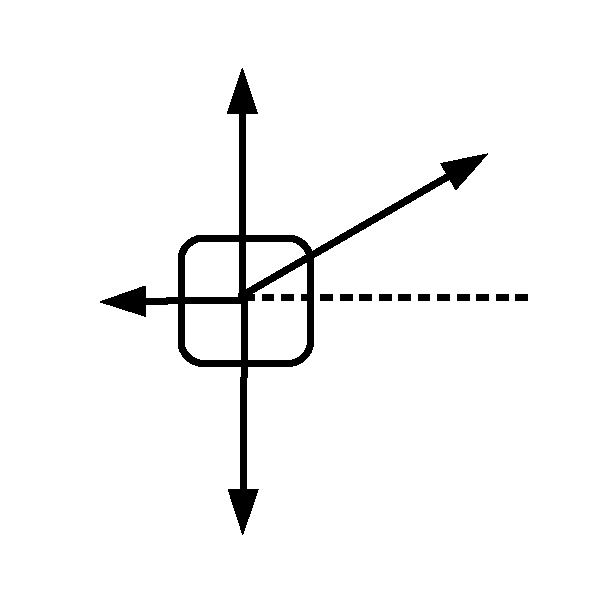
\includegraphics[width=0.3\textwidth]{figures/FBD1.pdf} \\
(b) Calculate the work done on the the system if the mass is 100 kg, $\vec{x} = 1 \hat{i}$ m, the friction force is $-100\hat{i}$ N, and the magnitude of $\vec{F}$ is 400 N. \textbf{Solution}: The net force in the x-direction (the direction of the displacement) is $-100 + 200\sqrt{3}$ N, so the force times the displacement is $100(2\sqrt{3}-1)$ J.
\end{enumerate}
\section{Kinetic Energy}
\begin{enumerate}
\item What is the kinetic energy of a system with mass 2 kg moving at $\sqrt{10}$ m/s? \textbf{Solution}: $KE = \frac{1}{2}mv^2 = \frac{1}{2}(2)(\sqrt{10})^2 = 10$ J.
\item What would be the kinetic energy if the speed doubled?  \textbf{Solution}: Kinetic energy is proportional to the square of the speed, so if we double speed the kinetic energy quadruples: KE = 40 J. \textit{This is an example of a \textbf{scaling} problem}.
\end{enumerate}
\section{Work-Energy Theorem}
\begin{enumerate}
\item How much work is required to compress a spring with spring constant $k = 500$ N/m by a displacement 0.1 m?  How high will an object go if we use the spring to shoot something straight up, if it has 0.1 kg mass?  \textbf{Solution}: $W_{\rm s} = \frac{1}{2}kx^2 = \frac{1}{2}(500)(0.1)^2 = \frac{5}{2}$ J.  As for the height, we can solve it kinematically, but it's much easier to use gravitational potential energy: $PE = mgh$, so $\frac{5}{2} = 0.1 * 10 h$, or $h = \frac{5}{2}$ m.
\end{enumerate}
\section{Gravitational Potential Energy}
\begin{enumerate}
\item What is the maximum velocity achieved by an object if we drop it from 300 m?  (No drag).  \textbf{Solution}: Set gravitational potential energy equal to kinetic energy and solve for speed: $PE = KE$, so $mgh = \frac{1}{2} m v^2$, or $v = \sqrt{2gh} = \sqrt{2*10*300} = \sqrt{6000}$ m/s (about 80 m/s).
\end{enumerate}
\section{Conservative Forces}
\begin{enumerate}
\item Be able to describe, in your own words, what is a conservative force.  Which of these forces is conservative?  (a) Friction, kinetic (b) Drag, air (c) Stoke's Law (drag in viscous liquids) (d) Hooke's Law
\end{enumerate}
\end{document}